\chapter{界面设计}
\section{客户端界面}
\vspace{3ex}
\begin{figure}[H]
	\centering
	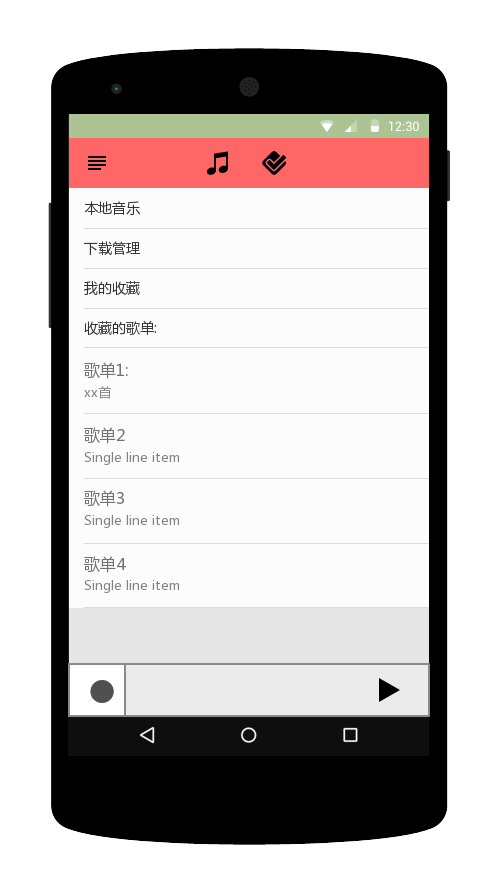
\includegraphics[width=10cm]{kehuduan.png}
	\caption{客户端界面} 
	\label{fig:figure8}
\end{figure}


这里是用户打开应用程序时的界面,界面分为两部分:主页面和播放栏.


播放栏在大部分情况下都会存在,是一个长久存在的ui组件,用于对播放状态进行控制,用户可以点击播放按钮,控制当前按钮的播放.或者通过点击位于播放栏左侧的图标,进入歌曲详情界面.对于歌曲详情界面,下面会进行展示


主页面是一个包含两项的ViewPager,其中第一个页面(左边的页面)是我的音乐界面栏.用户可以通过点击相应选型进入其他界面:
\begin{itemize}
	\item 最近播放:进入最近播放界面
	\item 下载管理:进入下载管理界面
	\item 我的收藏:进入我的收藏界面
	\item 歌单X:进入歌单界面
\end{itemize}

用户可以点击标题栏右边的按钮进入动态主页界面.

用户可以通过点击标题栏最左侧的列表按钮,或者从左向右进行拖拽打开用户选项栏


\section{登录界面}
\begin{figure}[H]
	\centering
	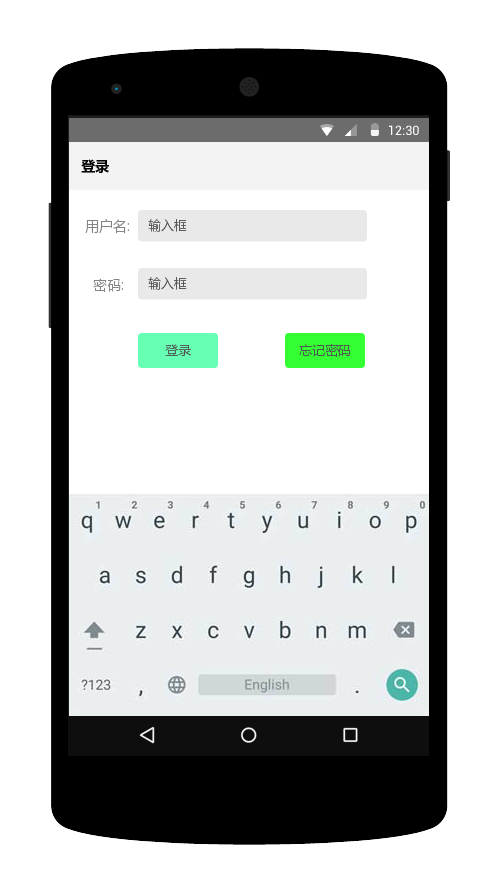
\includegraphics[width=10cm]{denglu.png}
	\caption{登录界面} 
	\label{fig:figure1ss8}
\end{figure}

在用户登录界面,用户在输入框中输入用户名及密码,点击登录按钮后即可完成登陆操作.如果登录成功,返回客户端界面,否则,留在登录界面,显示错误信息.如果用户点击忘记密码按钮,则调用系统的WebView访问预设的密码更改页面.

\section{播放界面}

\begin{figure}[H]
	\centering
	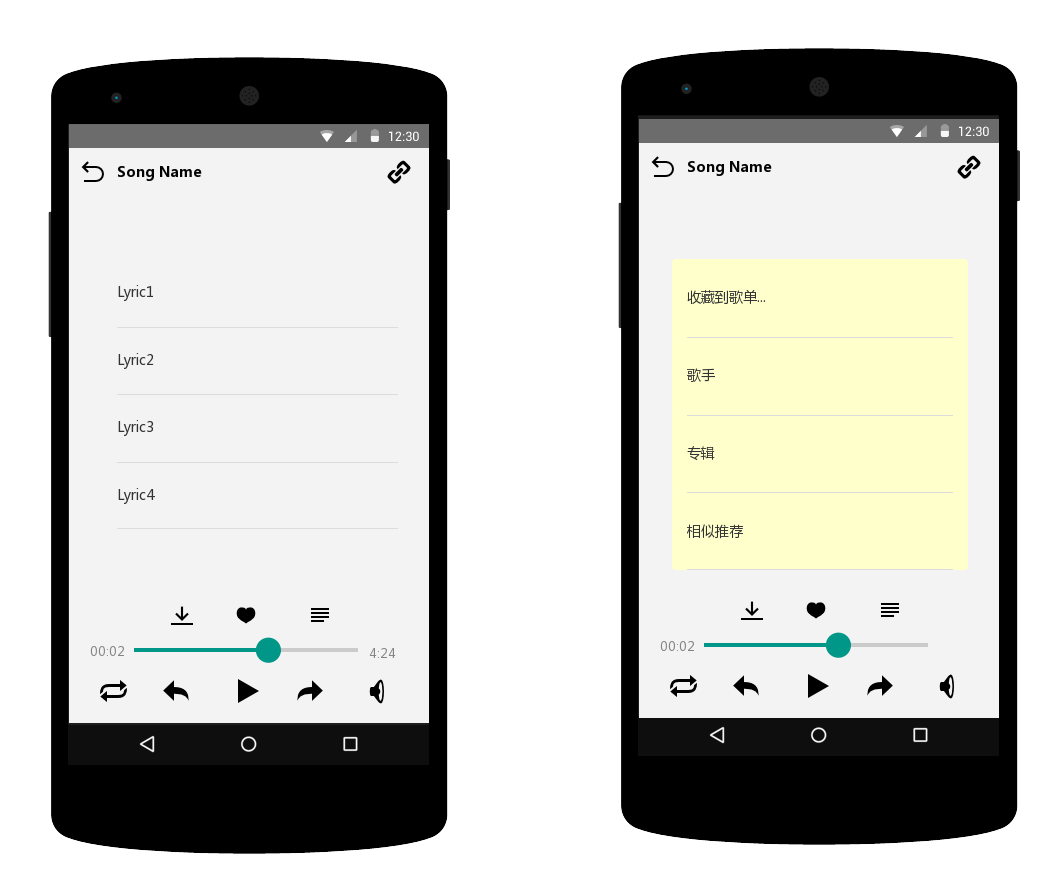
\includegraphics[width=10cm]{bofang.png}
	\caption{播放界面} 
	\label{fig:figure1s8}
\end{figure}

用户通过点击歌曲项进入播放界面时,将进入左图所示的歌曲界面.用户通过点击界面上的按钮将进行不同操作
\begin{itemize}
	\item 标题栏左边的返回按钮:将返回上一个活动
	\item 标题栏右边的链接按钮:进行分享操作,其行为由系统定义
	\item 底层
\end{itemize}	



底层栏:
\begin{itemize}
	\item 最左侧循环按钮:切换播放方式,包括列表循环等
	\item 上一首:播放上一首歌曲
	\item 播放/暂停:进行歌曲的播放/暂停,图标相应发生变化
	\item 下一首:播放下一首歌曲
	\item 喇叭:设置播放音量
\end{itemize}


进度条:
\begin{itemize}
	\item 进度条:用户通过拖动进度条控制播放进度
\end{itemize}



进度条上方栏:
\begin{itemize}
	\item 下载按钮:下载当前歌曲
	\item 收藏按钮:将当前歌曲加入/删除到"我最喜爱的歌曲"歌单中
	\item 选项按钮:展开选项栏,效果如右图所示
\end{itemize}



展开的选项栏:
\begin{itemize}
	\item 收藏到歌单:收藏到选定的用户歌单中
	\item 歌手:打开该歌手界面
	\item 专辑:打开该专辑界面
	\item 相似推荐:打开相似推荐界面
\end{itemize}


\section{专辑界面}

\begin{figure}[H]
	\centering
	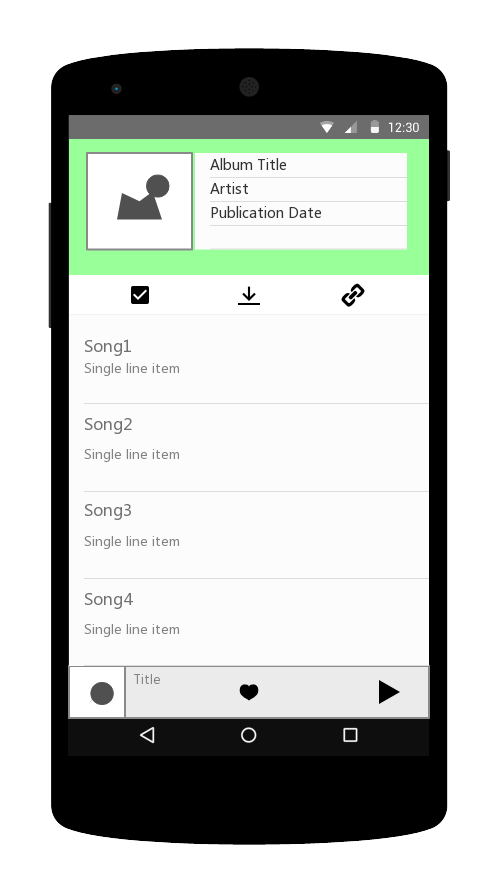
\includegraphics[width=10cm]{zhuanji.png}
	\caption{专辑界面} 
	\label{fig:figure118}
\end{figure}

专辑界面显示了一个专辑的基本信息,包括专辑封面,专辑名称,歌手,发行日期等信息,同时,以歌曲项列表的形式显示专辑内的所有歌曲.
底部播放栏前面已经介绍,不再赘述.

\begin{itemize}
	\item 选择按钮:用户点击后可以选择将专辑内所有歌曲加入指定歌单中
	\item 下载按钮:用户点击后可以下载专辑内所有歌曲
	\item 分享按钮:用户点击后可以将专辑分享给其他应用,行为由系统确定.
\end{itemize}

\section{歌单界面}
歌单界面显示了一个歌单的基本信息,其界面和专辑界面类似,但是没有歌手,发行日期信息,其他行为表现和专辑界面完全一致,不再赘述.

\section{歌手界面}
\begin{figure}[H]
	\centering
	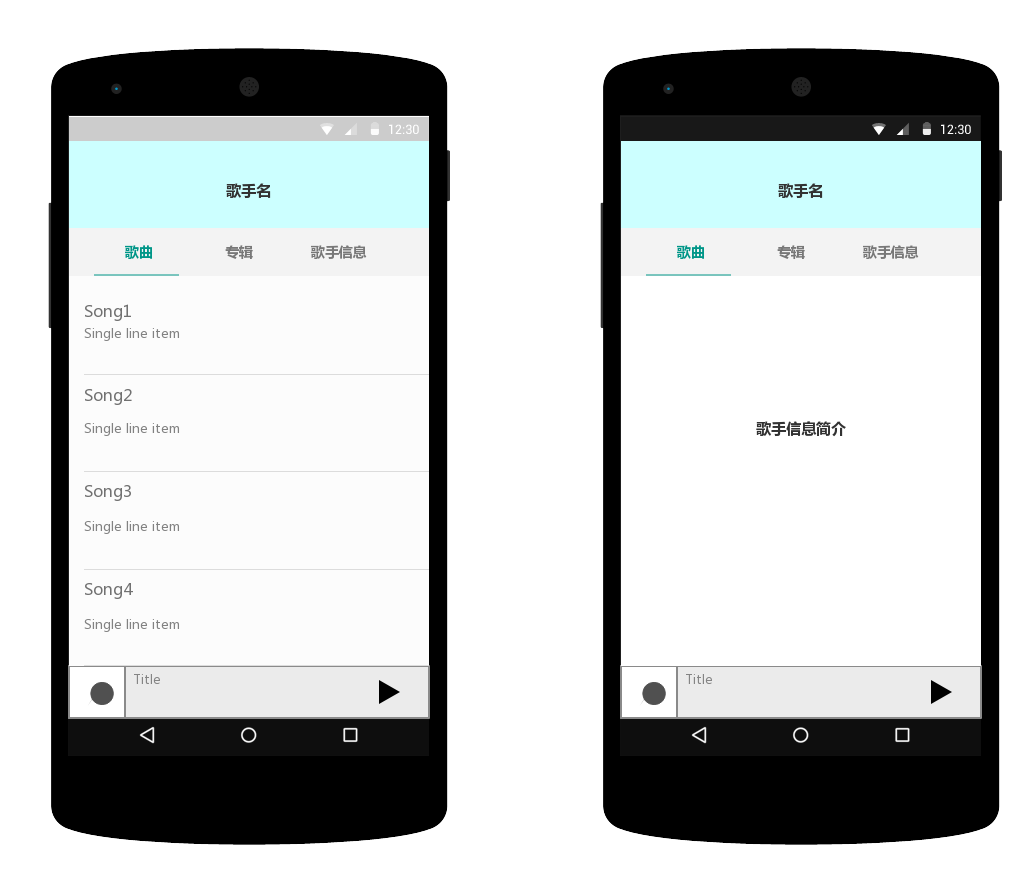
\includegraphics[width=10cm]{geshou.png}
	\caption{歌手界面} 
	\label{fig:figure1v8}
\end{figure}

用户可以在三个选项卡内进行选择,可以找到该名歌手的所有歌曲,所有专辑和歌手简介三个页面.

\begin{itemize}
	\item 所有歌曲界面:用户通过点击某一歌曲项,可以进入该歌曲的歌曲界面
	\item 所有专辑界面:用户通过点击某一专辑项,可以进入该专辑的专辑界面
	\item 歌手简介界面:只显示简介文本
\end{itemize}

